
\documentclass{egpubl}
\usepackage{eurovis2021}

\EuroVisShort  %

\usepackage[T1]{fontenc}
\usepackage{microtype}
\usepackage{dfadobe}  

\usepackage{cite}  %
\BibtexOrBiblatex
\electronicVersion
\PrintedOrElectronic
\ifpdf \usepackage[pdftex]{graphicx} \pdfcompresslevel=9
\else \usepackage[dvips]{graphicx} \fi

\usepackage{egweblnk}

\usepackage{csquotes}

% Allow for subcaptions:

% Replicate styling of figure caption labels and texts
\usepackage[labelfont=bf,textfont=it]{caption}
\usepackage[labelfont=bf,textfont=normalfont]{subcaption}

% Allow for strikethrough text using \sout{}
\usepackage[normalem]{ulem}

% CUSTOM PACKAGES
\usepackage{tikz}
\usetikzlibrary{calc,positioning,spy}

\title[RoomCanvas: A Visualization System for Spatiotemporal Temperature Data]%
{RoomCanvas: A Visualization System for\\Spatiotemporal Temperature Data in Smart Homes}

\author[B. K{\"o}nig et al.]%
{\parbox{\textwidth}{\centering 
        B. K{\"o}nig~\orcid{0000-0002-8113-7863}, %
     	D. Limberger~\orcid{0000-0002-9111-4809}, 
        J. Klimke~\orcid{0000-0002-4650-711X},
        B. Hagedorn~\orcid{0000-0001-9315-9333}, and 
        J. D{\"o}llner
    }
    \\
 	{\parbox{\textwidth}{\centering %
        Hasso Plattner Institute, Digital Engineering Faculty, University of Potsdam, Germany
    }}
}

\usepackage{eso-pic}
\setlength{\paperwidth}{210mm}\setlength{\paperheight}{297mm}% egpubl leaves them 0; needed by eso-pic
\AddToShipoutPictureFG{\AtPageLowerLeft{\put(\LenToUnit{0.5\paperwidth},\LenToUnit{6mm}){\makebox[0pt][c]{\fontsize{6.5}{8}\selectfont\color{gray}Author's revised version (2026-11-08). Version of record: https://doi.org/10.2312/evs.20211048}}}}
\begin{document}

\teaser{
  \centering
  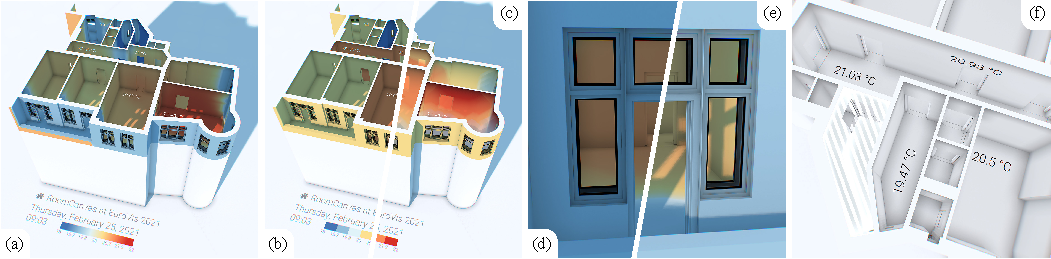
\includegraphics[width=\linewidth]{figures/figure-1-overview_images-embedded-v5.pdf}
  \caption{%
  RoomCanvas depicting data from multiple temperature sensors of an apartment using a diverging color scale: (a)~interpolated and projected to walls, floors, and ceilings, (b)~aggregated per-room, or (c)~displayed using volumetric rendering. Our interpolation has spatial awareness of room-boundaries, doors, and windows. % 
  (d) and (e) showcase the geometric detail and different times of day, enabling indoor views and recognizable structural elements. (f) shows our adaptive label positioning and interactive highlighting of rooms. %
  Sun position and lighting are simulated for the time and day at the geographic position in (a) to (e) and the outside temperature is taken into account as well.%
  }
  \label{fig:teaser}
}

\maketitle

\begin{abstract}
    Spatiotemporal measurements such as power consumption, temperature, humidity, movement, noise, brightness, etc., will become ubiquitously available in both old and modern homes to capture and analyze behavioral patterns. 
    The data is fed into analytics platforms and tapped by services but is generally not readily available to consumers for exploration due in part to its inherent complexity and volume. 
    We present an interactive visualization system that uses a simplified 3D representation of building interiors as a canvas for a unified sensor data display. 
    The system’s underlying visualization supports spatial as well as temporal accumulation of data, e.g., temperature and humidity values. 
    It introduces a volumetric data interpolation approach which takes 3D room boundaries such as walls, doors, and windows into account. We showcase an interactive, web-based prototype that allows for the exploration of historical as well as real-time data of multiple temperature and humidity sensors. 
    Finally, we sketch an integrated pipeline from sensor data acquisition to visualization, discuss the creation of semantic geometry and subsequent preprocessing, and provide insights into our real-time rendering implementation.
\begin{CCSXML}
<ccs2012>
   <concept>
       <concept_id>10003120.10003145.10003151.10011771</concept_id>
       <concept_desc>Human-centered computing~Visualization toolkits</concept_desc>
       <concept_significance>300</concept_significance>
       </concept>
   <concept>
       <concept_id>10003120.10003145.10003151</concept_id>
       <concept_desc>Human-centered computing~Visualization systems and tools</concept_desc>
       <concept_significance>500</concept_significance>
       </concept>
   <concept>
       <concept_id>10003120.10003145.10003147.10010923</concept_id>
       <concept_desc>Human-centered computing~Information visualization</concept_desc>
       <concept_significance>500</concept_significance>
       </concept>
 </ccs2012>
\end{CCSXML}
    
    \ccsdesc[300]{Human-centered computing~Visualization toolkits}
    \ccsdesc[500]{Human-centered computing~Visualization systems and tools}
    \ccsdesc[500]{Human-centered computing~Information visualization}
    
    \printccsdesc
    
\end{abstract}  

\begin{figure*}[t]
    \centering
    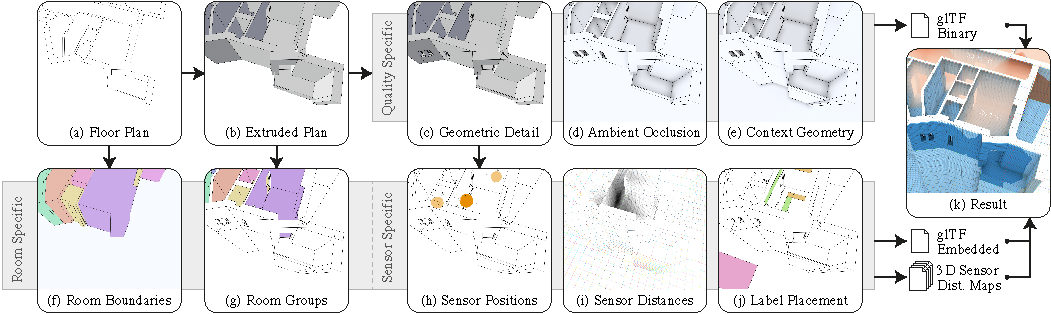
\includegraphics[width=\linewidth]{figures/figure-2-components_embedded-v4.pdf} 
    \caption{From a given (a) floor plan, a (b) simplified 3D apartment representation is created via extrusion, which is then used for further preprocessing to increase visual quality and to compute and store data attributes: (c) detailed geometry is added, (d) ambient occlusion is prerendered, and (e) a block for lower floors—indicating the apartment’s floor level—and a ground plane are added. 
    At the same time, (f) floor-plan-based extrusion of simplified meshes representing the individual rooms' boundaries, (g) assignment of faces to the corresponding room surfaces, and (h) configuration of the sensors’ positions allow for corresponding aggregations and interaction events. For each sensor, (i) distances to every point in a discretized volume spanning the apartment's bounding box are precomputed using a three-dimensional flood fill variant and encoded in 3D textures, and (j) candidates for dynamic label placement are precalculated. 
    (k) Based on the outputs of those preprocessing steps, our visualization can interpolate, display, and label sensor data at interactive frame rates (even on smartphones).}
    \label{fig:visualization-components} 
\end{figure*}

\section{Introduction}
The living comfort in apartments and houses depends, among other factors, strongly on the thermal comfort of the occupants and thus on the thermal environment indoors~\cite{ye2012-ambient,yun2020-indoor}.
The availability of low-cost, low-energy, and easy-to-install IoT-enabled sensors has simplified data monitoring and data gathering for consumers.
Thus, we need effective tools to explore, monitor, and understand such measurements in their spatial and temporal context.
The temporal aspect of collected temperature data requires applying temporal visualization techniques, such as line graphs with a calendar/week/month selection---but those techniques are usually limited to this temporal dimension alone and do not take spatial relations into account. %
The spatial propagation of heat in buildings creates the need to apply visualization techniques for spatial data, such as heat maps with a per-building or per-floor aggregation—often lacking a graphical connection to the building’s structure. %
The spatial structure, however, is also often already readily available for newly built buildings due to the increased integration of \emph{building information modeling} (BIM) techniques and standards, and allows for interesting and insightful visual display of temperature and humidity.

We propose 
an interactive, web-based, real-time 3D 
visualization system, called \emph{RoomCanvas}, that is built around the spatial nature of buildings, apartments, and rooms. It allows for the visualization of spatiotemporal data directly at its respective location, employing techniques such as spatial and temporal interpolation, color mapping, and automated label placement. 
As opposed to existing, expert-targeted BIM simulation and visualization software systems~\cite{chang2018-automated}, which focus on being mechanically precise and use sufficiently aesthetic models of building structures and contents, we chose to build a system for a broader target audience.
Available systems typically do not interpolate sensor values spatially~\cite{delgado2018-structural,mccaffrey2015-development}, are not or only partially web-based~\cite{mccaffrey2015-development}, and in some cases tightly integrated with existing expert tools such as Revit.
To this end, we have slightly different design goals, namely, the suitability for web-based, real-time rendering, a focus on increased aesthetic quality and recognizability using a sufficiently precise model representation of the built environment, and interaction tools targeted towards non-experts.

\section{Data Provisioning and 3D Floor Plan Modeling}%
\label{sec:Data Processing and Provisioning}

Our visualization relies on (1) access to real-time or historic temperature data as much as on (2) an accurate and up-to-date 3D floor plan with (3) room semantics, (4) preferred locations for view-dependent labeling, and, finally, (5) precomputed spatial distance data for every data source, i.e., every single sensor.

\paragraph*{Temperature Data Integration}
For our measurements, we combine multiple sensors for temperature, humidity, and atmospheric pressure (inside and outside, usually one per room), with sensors for opening states of windows and doors based on the wireless, low-energy ZigBee protocol, as well as public weather services for outside temperature tracking.
The sensors are connected to a ZigBee gateway (Raspbee) on a Raspberry Pi %
 running deCONZ home automation software.
Node-RED is then used to filter, transform, and transmit raw sensor data to a real-time data analytics platform via the MQTT protocol. %
There, the sensor data is semantically structured, analyzed as needed, and stored for efficient provision via authorized API requests.
Additional data resources can be and---in the case of outside weather information---are added and integrated here.
In addition to raw data access, the analytics platform API supports requests for custom data resolutions, time ranges, accumulations, filtering, and more. 
This, for example, allows querying time series as complex as the daily average in temperature around noon for every March of the last five years (assuming data was collected for that time span, obviously).%

\paragraph*{Drawing of 3D Floor Plans}

One of our main concerns when designing our 3D visualization was to prevent visual clutter from the beginning.
Instead of using 3D LiDAR scans, photogrammetry, or complex CAD drawings, we model, enhance and optimize the 3D geometry ourselves.
To this end, we create a minimal but accurate floor plan (\autoref{fig:visualization-components}~(a)), extrude walls, add ceilings and floors, account for special areas such as balconies, steps, etc., and finally, add doors and windows.
During the whole process, we keep the number of faces and vertices as low as reasonably possible.

To increase the authenticity of our floor plans, to provide a reference to the location of the apartment in its surrounding building (context), and to reduce the rendering complexity at run-time, we precompute a light map, e.g., accounting for local ambient occlusion~\cite{akenine2018}~(\autoref{fig:visualization-components}~(d)) and add a low-polygon representation of lower floors and (optionally) the immediate environment~(\autoref{fig:visualization-components}~(e)).
Furthermore, we compute the sun position~\cite{kolivand2011-realtime} and approximate physically plausible soft shadows~\cite{molzer2019-interactive} in real-time using multi-frame sampling~\cite{limberger2017-progressive}.

\paragraph*{Semantic Enrichment of 3D Floor Plans}

We group every polygon of the geometry into semantic units and layers such as lateral walls, ceilings, floors~(\autoref{fig:visualization-components}~(f--g)). 
To allow for user interaction with individual rooms, we apply a naming scheme and finally store everything as a glTF model.
Applying this process enabled us to understand the optimal characteristics of the 3D model and to identify techniques for its semi-automated computation in the future.

\begin{figure}[t]
    \centering
    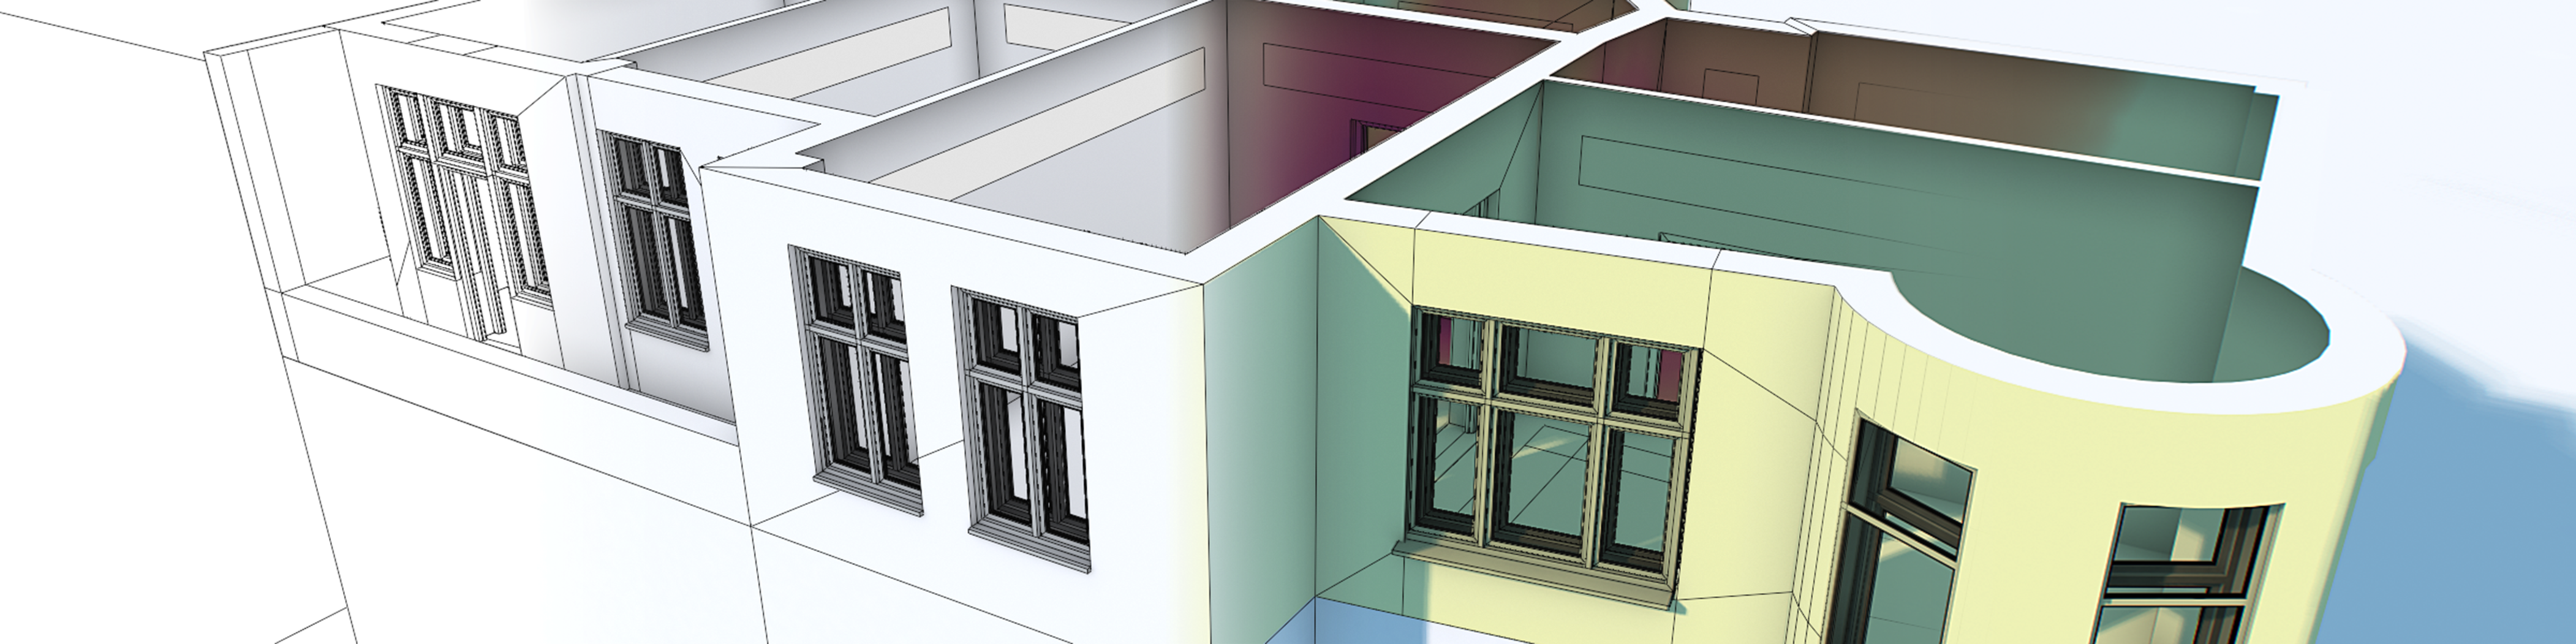
\includegraphics[trim=96 0 96 0, clip, width=\linewidth]{figures/figure4.png} 
    \caption{An optimized, low-polygon 3D floor plan, enhanced with precomputed ambient occlusion maps and real-time shadows to serve as a canvas for the visual display of interpolated sensor values.} %
    \label{fig:overview-about-3d-floor-plan-rendering} 
\end{figure}

\paragraph*{Per-Sensor Distance Map Computation}

To enable spatially unrestricted sampling of temperature values in 3D, we use precomputed 3D distance maps (distance volume) for every single sensor~(\autoref{fig:visualization-components}~(i)).
A distance volume encodes, at every cell (voxel), the shortest path to its sensor’s location in three dimensions, taking the complete geometry into account in 3D, i.e., walls, doors, windows, small openings, etc.
First, we create a cuboid with sufficient extent and reasonable resolution, i.e., the oriented bounding box of the 3D floor plan, and a voxel extent of, e.g., 10 to 20\,cm.
Second, we compute a binary 3D floor plan, storing whether or not a cell intersects with at least one polygon  (ceiling, floor, walls, etc.).
Finally, we use a modified flooding algorithm to create a 16\,bit distance map per sensor.
This needs to be done only once per sensor. 
Adding new sensors does not invalidate earlier distance maps, and only requires computing a single additional distance map.
Since WebAPIs do not have native support for 3D images, we use multiple distance maps---sliced into rows and columns of regular 2D images---encoded in one or more texture atlases.
Since there is no 16\,bit support either, the low and high bytes are spread over subsequent color channels.

\paragraph*{Computation of Preferred Label Locations}

We manually specify suitable locations for automated text placement~(\autoref{fig:visualization-components}~(j)). 
More specifically, we define rectangles within the 3D floor plan, primarily aligned to floors and upper parts of lateral surfaces.
We apply the naming scheme we used for the rooms to the rectangles and store them in an extra layer within the glTF assets.
While loading the rectangles, label locations are derived, based on a starting point, an up vector, a forward-facing vector, and a text running direction with its length encoding the maximum possible text length.

\paragraph*{Outside Temperature}

Additional temperature sensors that are placed outside can provide spatial temperature information to points of interest (terrace, balcony, etc.) and, furthermore, can help to differentiate between opposite exterior facades (e.g., drafts).
To establish a baseline for outside temperature, we use data available through open weather APIs, i.e., OpenWeatherMap.
If no geographic location is available, heat transfer depending on type and structure of the windows could be calculated and integrated as a data source~\cite{arici2015-flow}.
However, we assume a uniformly distributed temperature for the entire outdoor area, since the correctness of our interpolation is not sufficiently verified.

\section{Visualization}

Our proposed visualization system 
combines the idea of visualizing sensor data in building models\cite{chang2018-automated} with spatial aggregation and interpolation methods, such as inverse distance weighting (IDW)\cite{shepard1968-two}.
Therein, we use the base 3D building model as a canvas for direct in-place visualization of values~(\autoref{fig:overview-about-3d-floor-plan-rendering}).

\paragraph*{Per-Room Display} 

To provide insights on a room level basis, i.e., to allow for a fast judgment of the temperature distribution at a given time across a building’s rooms, our system combines all sensor measurements from inside a room into one mean value per room, which is then mapped via a color mapping and rendered on all walls, the floor, and the ceiling of the corresponding room~(\autoref{fig:teaser}~(b)).

\paragraph*{Fine-grained Spatial Interpolation} %
 
To allow for a more fine-grained analysis of the approximated temperature distributions in a building at a given time, we use a spatial interpolation method.
\autoref{fig:teaser}~(a) shows an example for this interpolation:
For each position on the projected-to surface, our system uses the distances to each sensor in the building for weighting the corresponding sensor value’s influence on the resulting encoded value using IDW. 
To increase the quality of the spatial interpolation, advanced spatial interpolation methods such as Kriging\cite{oliver1990-kriging}---which has already been successfully applied in interpolating sensor data inside buildings\cite{li2018-spatiotemporal}---could be integrated into our visualization system. 

\paragraph*{Volumetric Display} 

For the volumetric visualization of interpolated sensor data (\autoref{fig:teaser}~(c)), we use a ray-marching-based approach of tracing through the rooms’ volumes up to their respective back-faces (\autoref{fig:visualization-components}~(g)) and aggregating the sampled, interpolated sensor values along the way.
At each sampled volume location, we again color-map the respective interpolated sensor value to an RGB color value using the selected color scale, while at the same time using a configurable opacity transfer function to determine the sample’s opacity.
We then accumulate the samples using a standard front-to-back compositing equation and progressively enhance the visual quality of the volume rendering by shifting a pseudo-randomly generated hash used for jittering, and by adaptively increasing the sampling resolution. 

\paragraph*{Dynamic Label Placement} 

For dynamic rendering and placement of three-dimensional text labels we use OpenLL~\cite{limberger2018-openll} in combination with our precomputed label locations. 
This allows for algorithmic optimization of the most suitable position, orientation, and length for the to-be-displayed labels, taking into account the camera’s position as well as visibility and size constraints.
Our system first filters potential label placement positions by a set of criteria based on their orientation (front-facing normal points towards camera; text is readable from left-to-right in screen space co-ordinates) and position (label position is not obstructed by any geometry, determined by sampling the depth buffer; label’s world position transformed to screen space co-ordinates is within the view frustum). 
Then, we sort the remaining potential placement positions using a set of comparison attributes, such as the label’s size, its distance to the camera, and the angle between the label’s front-facing normal and the vector from the camera’s eye to the label’s position. 

\section{Results \& Discussion}

The results of our work include exemplary static, dynamic, and interactive visualization artifacts for the sample apartment, as well as the design and implementation of an end-to-end system for data measurement, collection, aggregation, and visualization. 
With the implementation of a prototypical, web-based viewer, we aim to provide a basis for extensions of the proposed visualization system and for experimentation in related use case areas.

\begin{figure}[t]
    \centering
    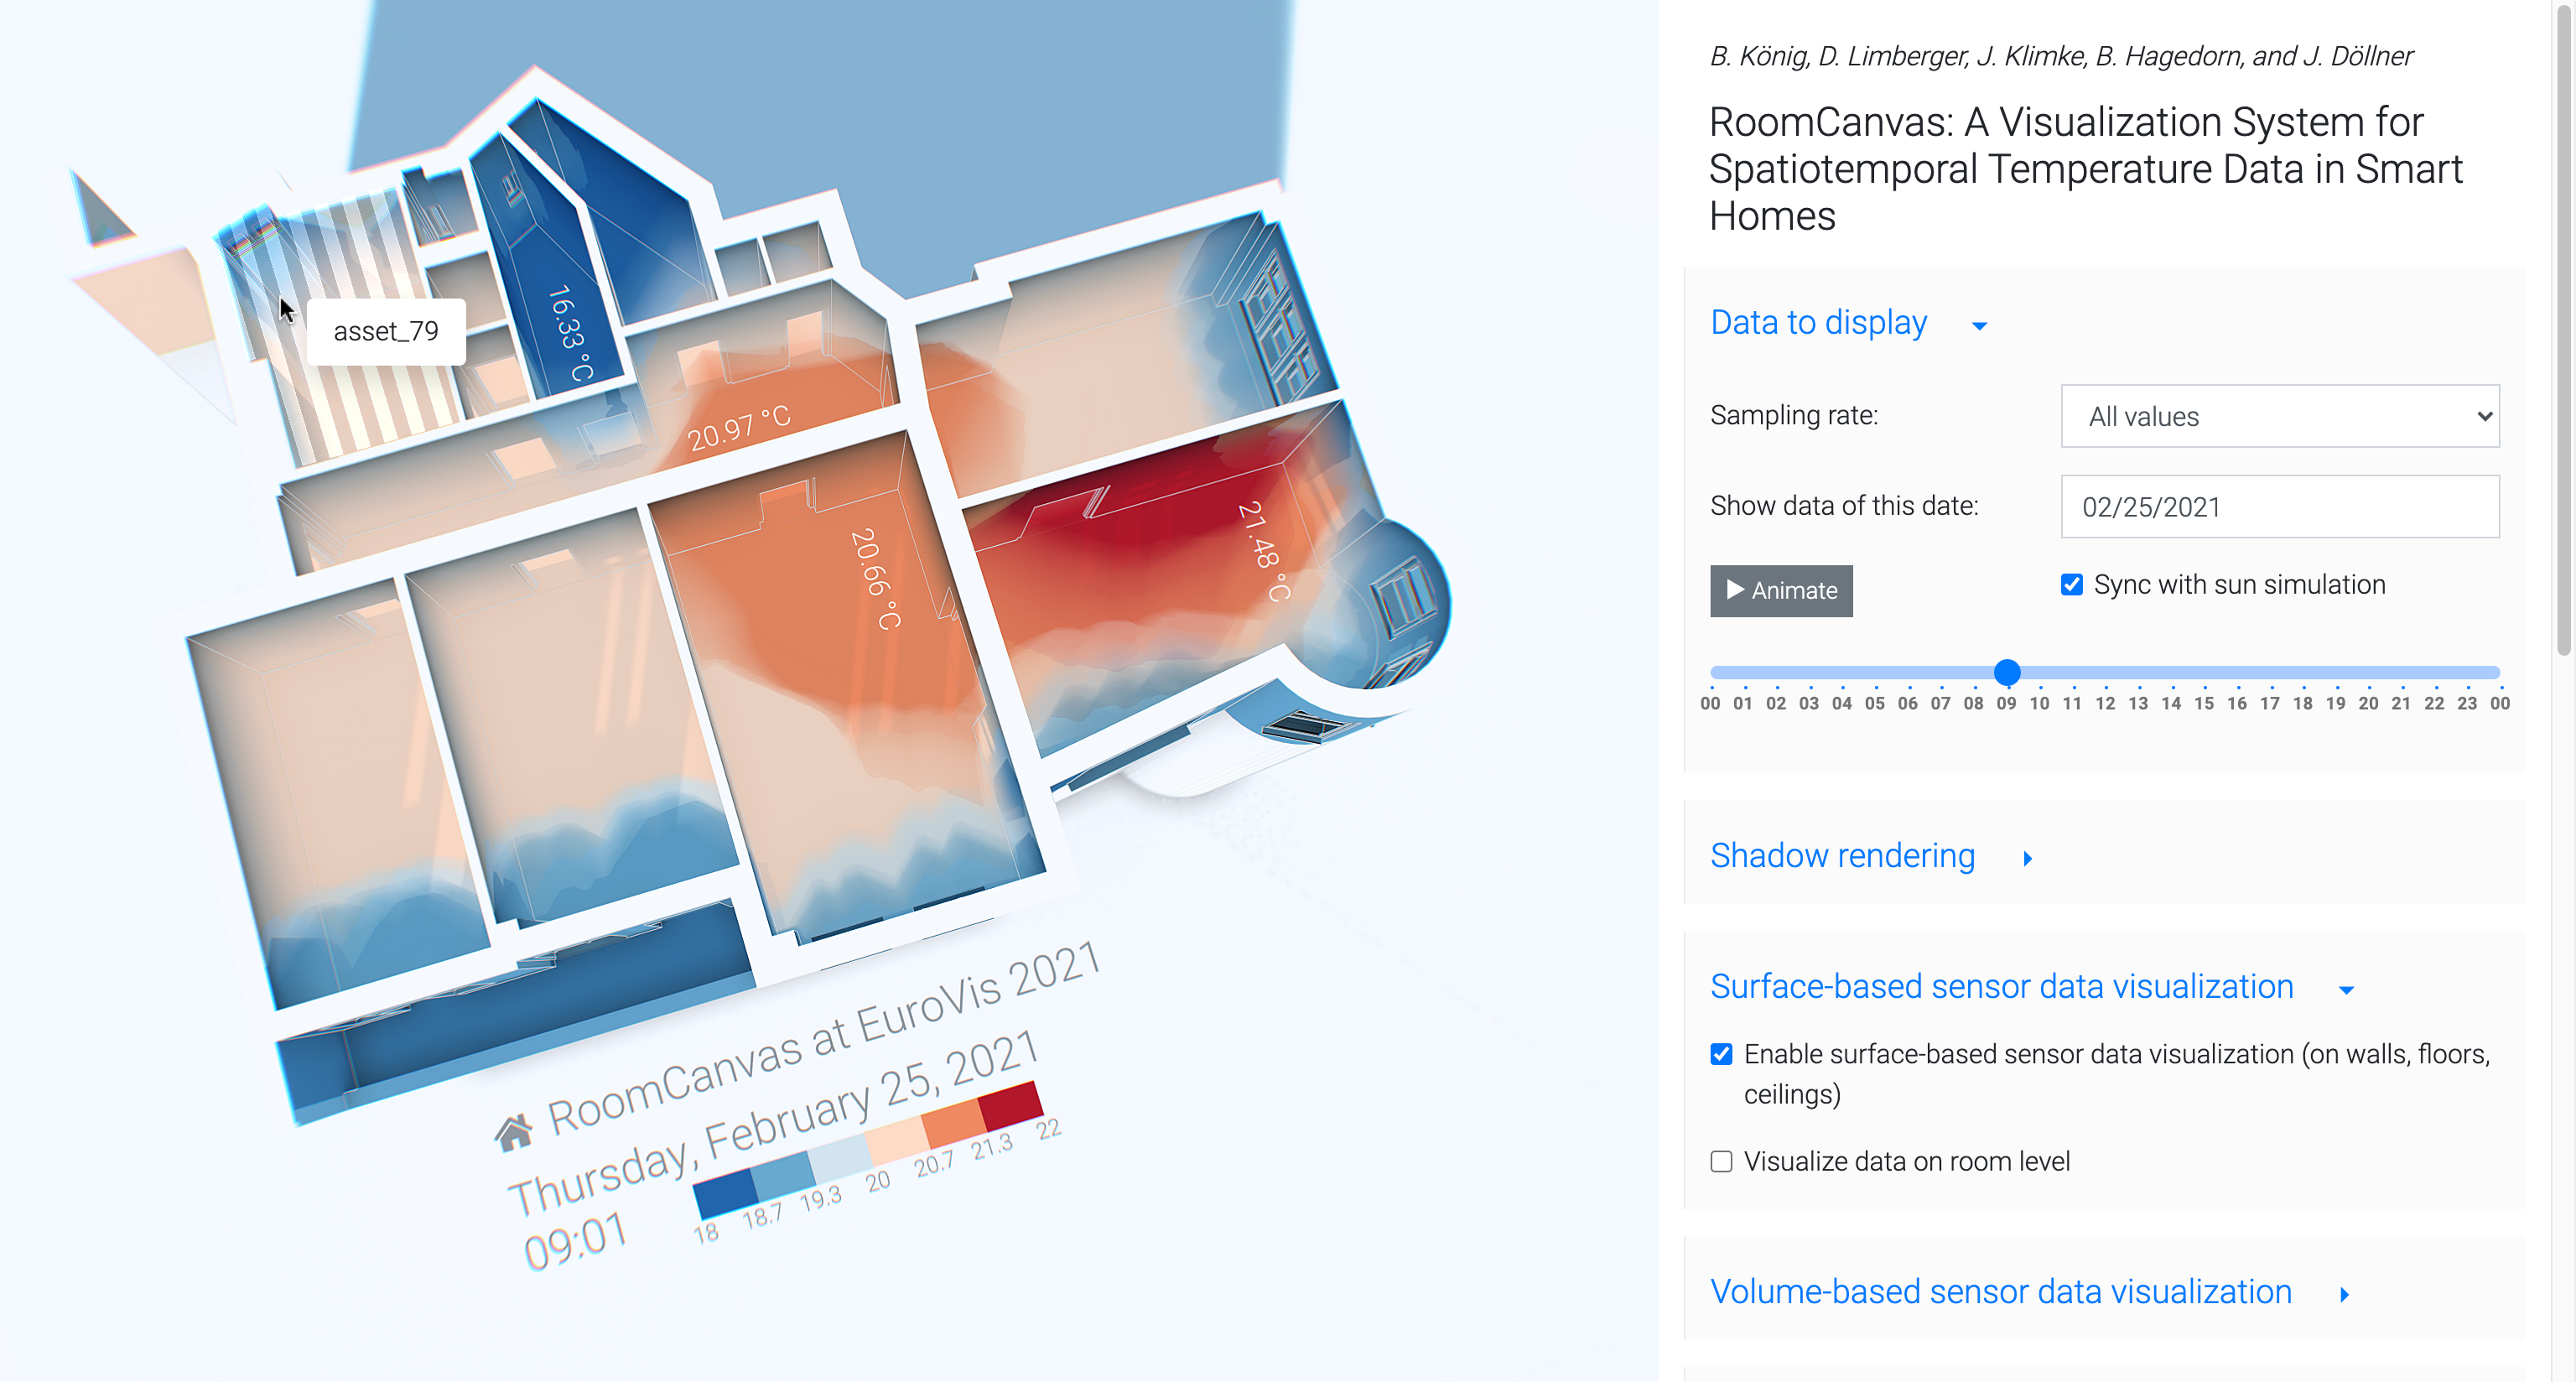
\includegraphics[trim=0 0 0 0, clip, width=\linewidth]{figures/figure-3-ui-screenshot-cropped-v4.png} 
    \caption{The interactive, web-based, real-time visualization prototype allows for selecting time aggregation intervals and ranges, for animating historical data, for configuring the type, steps, and discretization of the used color scale, for navigating the 3D scene, and for interacting with elements of the building model.}
    \label{fig:ui-screenshot} 
\end{figure}

\paragraph*{Static Visualizations}

Still images allow for analysis of spatial distributions of temperature values~(\autoref{fig:teaser}).
Different spatial levels of detail, e.g., per-room or spatially interpolated, as well as different time-based aggregations are available for exploration. 
This already provides a promising stand-alone or complementary visualization for communicating temperature distributions in living scenarios.

\paragraph*{Animated Visualizations}

As an extension of static visualizations, animations can be created based on the proposed visualization system, e.g., by letting the visualized timestamp slide through days or hours, or by moving the camera along a path for insights into different areas. 
Therein, the use of shadow mapping improves the perception of seasonal and daily time differences.

\paragraph*{Sample Use Case}

One possible use case for RoomCanvas is to determine in which areas of an apartment (either abstracted to the room level, or freely on any given position) a certain temperature threshold is exceeded or fallen below, potentially averaged temporally over a certain time interval, such as in six-hour intervals. 
By combining the capability of RoomCanvas to precisely interpolate and display such data based on recorded temperature data with its ability of adding temporal and spatial context (through the simulated sun position, real-time rendered shadows, and recognizable visual details of the 3D floor plan), we aim to simplify such use cases---use cases which otherwise could possibly only be tackled by looking at 2D plots and charts and thus without spatial and temporal context.

\paragraph*{Interactive Visualizations}

Our work includes a prototype for an interactive, WebGL-based 3D viewer~(\autoref{fig:ui-screenshot}, visit \httpAddr{//roomcanvas.dev} for a live demo of the prototype). 
By loading preprocessed assets---a \emph{glTF binary file} containing the presentation-focused, high-quality apartment model, a \emph{glTF embedded file} containing the apartment’s logical and hierarchical structure, and a set of 3D textures encoding precomputed, occlusion-aware distances to sensors---, and by fetching and interpolating data on-demand from the analytics platform API (\autoref{sec:Data Processing and Provisioning}), the viewer implements the proposed visualization system and allows for data querying, selection, navigation, and spatial interactions.

\section{Conclusion \& Future Work}

We have introduced a system for high-quality visualization of built environments that combines spatial and temporal aspects of a variety of sensor data. 
The system can be used to generate aesthetic still images as well as to provide interactive access to real-time sensor data.
The fusion of the 3D floor plan with the unified sensor data representation potentially facilitates exploration and correlation of temporal changes in data to past events and actions of occupants.

Following the development of the visualization system, further research needs to be conducted to extend this approach to be applied on larger buildings as well as industrial facilities that are modeled using complex data models and standards in CAD, BIM (\emph{IFC}), or city modeling (\emph{CityGML}). Here, the challenge is how to scale the solution to support those large-scale models in terms of data processing, transmission, and rendering.
To make our system more accessible, one could simplify the currently manual process of drawing 3D floor plans, for example, by providing an export plug-in for consumer tools such as Sweet Home 3D. 

As related work provided promising approaches to finding the optimal number of sensors for a given location in other use case domains\cite{jedermann2009-minimum}, we believe that a minimum number of sensors can also be determined in an apartment or house, resulting in optimized resource usage while maintaining measurement quality.
The work described could further benefit from an optimized location sampling and an improvement in the placement of the sensors\cite{huang2015-sampling}, potentially in a semi-automated, assisted way.

\section*{Acknowledgements}
This work has been supported by the German Federal Ministry of Education and Research (BMBF) through grant 01IS19006  (\enquote{KI-Labor ITSE}).

\bibliographystyle{eg-alpha-doi}
\bibliography{references}

\end{document}

